\documentclass[UTF8,a4paper,12pt,scheme=chinese]{ctexbook}

\addtolength{\textwidth}{1in}
\addtolength{\hoffset}{-0.5in}
%\setlength{\voffset}{-1in}

\usepackage{amsmath}
\usepackage{amssymb}
\usepackage{textcomp} 
\usepackage{graphicx}
\usepackage{xcolor}
\usepackage{mathrsfs}
\usepackage{tikz}
\usepackage{amsthm}
%\usepackage{soul}
\usetikzlibrary{arrows,decorations.pathmorphing,backgrounds,positioning,fit,petri}

%\usepackage{latexsym}

\newcommand{\hlx}[2]{%
	\IfEqCase{#1}{%
		{1}{
			\colorbox{yellow!50}{$\displaystyle#2$}
		}
		{b}{
			\colorbox{yellow!50}{$\scriptstyle#2$}
		}
		{3}{
			\colorbox{yellow!50}{$\scriptscriptstyle#2$}
		}
	}
		% you can add more cases here as desired
	
}%


%\pagestyle{headings}
%\ctexset{

%}
\pagestyle{headings}
\ctexset{
%	section={	
%		name={第,章},
%		number=\arabic{section},
%	},
	section={
		name={第,节},
		number=\chinese{section},
	},
	subsection={
%		name={第,节},
		number=\chinese{subsection}、,
	},
	subsubsection/name = {},
	subsubsection={
%		name={asd,啊},
		number=\arabic{subsubsection}.,
		aftername={},
		format=\Large\bfseries\CJKfamily{zhsong},
	},
	paragraph={
%		name={asd,啊},
%		number=\arabic{subsubsection},
		format=\bfseries\youyuan,
	},
}
\setcounter{secnumdepth}{3}
\newcommand{\ud}{\mathrm{d}}
\newcommand{\lc}{\left(}
\newcommand{\rc}{\right)}

\newcommand{\hl}[1]{\colorbox{yellow}{#1}}
\newcommand{\hla}[1]{%
	\colorbox{yellow!50}{$\displaystyle#1$}}
\newcommand{\hlb}[1]{%
	\colorbox{yellow!50}{$\scriptstyle#1$}}
\newcommand{\hlc}[1]{%
	\colorbox{yellow!50}{$\scriptscriptstyle#1$}}

\makeatletter
\DeclareFontFamily{U}{tipa}{}
\DeclareFontShape{U}{tipa}{m}{n}{<->tipa10}{}
\newcommand{\arc@char}{{\usefont{U}{tipa}{m}{n}\symbol{62}}}%

\newcommand{\arc}[1]{\mathpalette\arc@arc{#1}}

\newcommand{\arc@arc}[2]{%
	\sbox0{$\m@th#1#2$}%
	\vbox{
		\hbox{\resizebox{\wd0}{\height}{\arc@char}}
		\nointerlineskip
		\box0
	}%
}

\everymath{\displaystyle}
%\newtheorem{btheorem}{b定理}[section]
\newtheorem{theorem}{定理}[section]
%\renewcommand{\theorem}{\arabic{subsection}.\arabic{thm}}
\newtheorem*{theorem*}{非书定理}
\theoremstyle{plain}
\newtheorem{definition}{定义}[section]
\newtheorem{property}{性质}[subsection]
\makeatother

\begin{document}
	\chapter{多元函数微分法及其应用}
	\section{多元函数的基本概念}
	\section{偏导数}
	\subsection{偏导数的定义及其计算法}
	\subsubsection{定义}
	\paragraph{一元函数}
	\begin{itemize}
		\item 导数
		\begin{enumerate}
			\item $f'(x_0) = \frac{\ud f}{\ud x}\Big|_{x=x_0}$
			\item $f'(x_0)=\lim\limits_{\Delta x \rightarrow 0}\frac{\Delta y(x=x_0\mbox{附近})}{\Delta x}$
			\item $f'(x_0)=\lim\limits_{\Delta x \rightarrow 0}\frac{f(x_0+\Delta x)-f(x_0)}{\Delta x}$
			\item $f'(x_0)=\lim\limits_{ x \rightarrow x_0}\frac{f(x)-f(x_0)}{x-x_0}$
		\end{enumerate}
		\item 导函数
		\begin{enumerate}
			\item $f'(x)=\lim\limits_{\Delta x \rightarrow 0}\frac{\Delta y(x\mbox{附近})}{\Delta x}$
		\end{enumerate}
	\end{itemize}
	\paragraph{二元函数}
	\begin{itemize}
		\item 偏导数
		\begin{enumerate}
			\item $f_x(x_0,y_0)=\frac{\partial z}{\partial x}\Big|_{
				\begin{subarray}{l}
				x=x_0\\
				y=y_0
				\end{subarray}}$
			\item $f_x(x_0,y_0)=\lim\limits_{\Delta x \rightarrow 0}
			\hla{\frac{f(x_0+\Delta x,y_0)-f(x_0,y_0)}{\Delta x}}$
			\item $f_x(x_0,y_0)=\frac{\ud f(x,y_0)}{\ud x}\Big|_{x=x_0}$(实质是一元函数的导数)
		\end{enumerate}
		\item 偏导函数
		\begin{enumerate}
			\item $f_x(x,y)=\frac{\partial z}{\partial x}$
			\item $f_x(x,y)=\lim\limits_{\Delta x \rightarrow 0}
			\frac{f(x+\Delta x,y)-f(x,y)}{\Delta x}(\overbrace{{\mbox{只与x,y有关}}}^{\mbox{是x,y的函数}}$,与$\Delta x$无关
		\end{enumerate}
	\end{itemize}
	\subsubsection{几何意义}
	\paragraph{$\tan x$}
	\subsubsection{可偏导与可连续}
	\paragraph{一元函数}
	可导必连续,连续不一定可导
	\paragraph{二元函数}
	偏导存在和连续\textbf{没有关系}
	\subparagraph{题目解释}
	\subparagraph{结构解释}
	\begin{enumerate}
		\item 偏导只有两个方向,而连续要求所有方向
		\item 一元函数的连续不一定可导
		\subitem eg.绝对值
	\end{enumerate}
	\subsection{高阶偏导函数}
	\subsubsection{类型}
	\paragraph{纯偏导函数}二元函数有两个
	\paragraph{混合偏导函数}二元函数有两个
	\subparagraph{写法}先x后y:$f_{xy}(x,y)=\frac{\partial^2 z}{\partial x \partial y}$
	\subsubsection{混合偏导的关系}
	\paragraph{充分条件}
	\begin{theorem}
		$f_{xy}(x,y),f_{yx}(x,y)$在D内连续$\Rightarrow f_{xy}(x,y)=f_{yx}(x,y)$
	\end{theorem}
	\begin{theorem}
		$
		f_{xy}(x,y)\Big|_{\begin{subarray}{l}x=x_0\\y=y_0\end{subarray}},
		f_{yx}(x,y)\Big|_{\begin{subarray}{l}x=x_0\\y=y_0\end{subarray}}$
		在$(x_0,y_0)$连续$\Rightarrow 
		f_{xy}(x,y)\Big|_{\begin{subarray}{l}x=x_0\\y=y_0\end{subarray}}=
		f_{yx}(x,y)\Big|_{\begin{subarray}{l}x=x_0\\y=y_0\end{subarray}}$
	\end{theorem}
	\begin{theorem}
		多元初等函数在其定义域上连续
	\end{theorem}
	\section{全微分}
	\subsection{全微分的定义}
	\subsubsection{增量}
	\paragraph{一元函数}~{}\\
	$\begin{array}{r c l l}
	\lim\limits_{ x \rightarrow x_0}f(x) & = & A\\ f(x)\big|_{x\rightarrow x_0}&=&A+o(\alpha) 
	\end{array}$
	\paragraph{二元函数}~{}\\
	\subparagraph{偏增量}~{}\\
	$\begin{array}{r c l l}
	\lim\limits_{\Delta x \rightarrow 0}
	\frac{f(x_0+\Delta x,y_0)-f(x_0,y_0)}{\Delta x} & = & f_x(x_0,y_0)\\
	\frac{f(x_0+\Delta x,y_0)-f(x_0,y_0)}{\Delta x}&=&f_x(x_0,y_0)+\alpha &(\lim\limits_{\Delta x \rightarrow 0}\alpha=0)\\
	f(x_0+\Delta x,y_0)-f(x_0,y_0)&=&f_x(x_0,y_0)\Delta x+\alpha\Delta x \\
	f(x_0+\Delta x,y_0)-f(x_0,y_0)&=&f_x(x_0,y_0)\Delta x+o(|\Delta x|) &(\lim\limits_{\Delta x \rightarrow 0}\frac{\alpha\Delta x}{\Delta x}=0)\\
	\Delta z(\mbox{偏增量})&=&f_x(x_0,y_0)\Delta x+o(|\Delta x|) \\
	\ud z(\mbox{偏微分})&=&f_x(x_0,y_0)\ud x
	\end{array}$
	\subparagraph{全增量}
	\subsubsection{定义}
	\begin{definition}~{}可微分,全微分
		\begin{itemize}
			\item 前提\quad$\exists A,B$与$\Delta x,\Delta y$无关,与$x,y$有关
			\item 条件
			\subitem 函数z在点$(x,y)$的全增量$\Delta z = f(x+\Delta x,y+\Delta y)-f(x,y)$\\可表示为
			$A\Delta x + B\Delta y +
			o(\rho)\quad(\rho = \sqrt{(\Delta x)^2+(\Delta y)^2})$
			\subitem 或
			\subitem $\lim\limits_{\rho \rightarrow 0}\frac{\Delta z - (A\Delta x + B \Delta y)}{\rho}=0$
			\item 结果
			\subitem z在点$(x,y)$可微分
			\subitem $A\Delta x + B\Delta y$为z在点$(x,y)$的全微分
			\subitem $\Delta z$不是全微分,是全增量,$\Delta z -o(p)$才是全微分
		\end{itemize}
		
	\end{definition}
	\subsubsection{可微的条件}
	\begin{theorem}
		可微$\Rightarrow$连续
		\begin{itemize}
			\item 证明\\
			$
			\begin{array}{r c l l}
				\lim\limits_{\begin{subarray}{l}
					\Delta x \rightarrow 0\\
					\Delta y \rightarrow 0
					\end{subarray}}
				f(x+\Delta x,y+\Delta y)&=&f(x,y)&(\mbox{由连续定义})\\
				\lim\limits_{\begin{subarray}{l}
					\Delta x \rightarrow 0\\
					\Delta y \rightarrow 0
					\end{subarray}}f(x+\Delta x,y+\Delta y)-f(x,y)&=&0\\
				\mbox{与此同时}&&\\
				\underbrace{f(x+\Delta x,y+\Delta y)-f(x,y)}_{
					\mbox{全增量}\displaystyle{\Delta z}
				}&=&A\Delta x + B\Delta y + o(\rho)&(\mbox{由前提})\\
				\lim\limits_{\begin{subarray}{l}
					\Delta x \rightarrow 0\\
					\Delta y \rightarrow 0
					\end{subarray}}f(x+\Delta x,y+\Delta y)-f(x,y)&=&\lim\limits_{\begin{subarray}{l}
					\Delta x \rightarrow 0\\
					\Delta y \rightarrow 0
					\end{subarray}}A\Delta x + B\Delta y + o(\rho)\\
				\lim\limits_{\begin{subarray}{l}
					\Delta x \rightarrow 0\\
					\Delta y \rightarrow 0
					\end{subarray}}f(x+\Delta x,y+\Delta y)-f(x,y)&=&0+0+0&(\mbox{高阶无穷小})\\
				\mbox{成立。}&&
			\end{array}
			$
			
			
		\end{itemize}
	\end{theorem}
	\begin{theorem}[必要条件]\hl{可微分的性质}
		~{}\\
		\begin{itemize}
			\item 前提\quad z在$(x,y)$可微分
			\item 结果 
			\subitem $ \exists $\textbf{偏导数}$z_x(x,y),z_y(x,y)$
			\subitem $z_x = A,z_y = B$
			\subitem $\ud z = z_x\Delta x+z_y \Delta y$
			\item 证明\\
			$
			\begin{array}{r c l l}
				\lim\limits_{\rho \rightarrow 0}\frac{\Delta z - (A\Delta x + B \Delta y)}{\rho}&=&0&(\mbox{由前提})\\
				\lim\limits_{\begin{subarray}{l}
					\Delta x \rightarrow 0\\
					\Delta y \rightarrow 0
					\end{subarray}}
				\frac{\Delta z - (A\Delta x + B \Delta y)}{\sqrt{(\Delta x)^2+(\Delta y)^2}}&=&0\\
				\mbox{沿y轴方向}&&\Delta y = 0\\
				\lim\limits_{
					\Delta x \rightarrow 0
				}
				\frac{\Delta z - (A\Delta x)}{\sqrt{(\Delta x)^2}}&=&0\\
				\lim\limits_{\Delta x \rightarrow 0}
				\frac{f(x+\Delta x,y)-f(x,y) - (A\Delta x)}{\sqrt{(\Delta x)^2}}&=&0\\
								\lim\limits_{\Delta x \rightarrow 0}
				\frac{f(x+\Delta x,y)-f(x,y) }{|\Delta x|}&=&\lim\limits_{\Delta x \rightarrow 0}\frac{ (A\Delta x)}{|\Delta x|}\\
				z_x & = & A
			\end{array}
			$
			
		\end{itemize}
	\end{theorem}
	\begin{theorem}[充分条件]
		\hl{可微分的条件}
		\begin{itemize}
			\item 前提
			\subitem \textbf{偏导数}$z_x(x,y),z_y(x,y)$存在,且\textbf{连续}
			\subitem 即
			\subitem$
			\begin{array}{r c l l}
			\lim\limits_{\begin{subarray}{l}
				\Delta x \rightarrow 0\\
				\Delta y \rightarrow 0
				\end{subarray}}
			f_x(x+\Delta x,y+\Delta y)&=&f_x(x,y)\\
			f_x(x+\Delta x,y+\Delta y)&=&f_x(x,y)+\alpha&(\lim\limits_{\begin{subarray}{l}
				\Delta x \rightarrow 0\\
				\Delta y \rightarrow 0
				\end{subarray}}\alpha = 0)
			\end{array}$
			
			\item 结果 
			\subitem z在$(x,y)$可微分
			\item 证明\\
			$
			\Delta z\\
			\begin{array}{lcll}
			=f(x+\Delta x,y+\Delta y)&-&f(x,y)\\
			=f(x+\Delta x,y+\Delta y)-f(x,y+\Delta y)&+&f(x,y+\Delta y)-f(x,y)&(\mbox{加减项})\\
			=f_x(\xi_1,y+\Delta y)(x+\Delta x-x)
			&+&
			f_y(x,\xi_2)(y+\Delta y-y)\\
			
			=f_x(\xi_1,y+\Delta y)\Delta x
			&+&
			f_y(x,\xi_2)\Delta y\\
			
			=f_x(x+\theta_1\Delta x,y+\Delta y)\Delta x
			&+&
			f_y(x,y+\theta_2\Delta y)\Delta y\\
			
			=[f_x(x,y)+\alpha]\Delta x
			&+&
			[f_y(x,y)+\beta]\Delta y&(\mbox{前提})\\
			
			=f_x(x,y)\Delta x+f_y(x,y)\Delta y
			&+&
			\alpha\Delta x+\beta\Delta y
			\end{array}\\
			$
			\\此时\\
			$
			\begin{array}{rcll}
			\lim\limits_{\rho \rightarrow 0}\frac{\alpha\Delta x+\beta\Delta y}{\rho} 
			& = &
			 \lim\limits_{\begin{subarray}{l}
				\Delta x \rightarrow 0\\
				\Delta y \rightarrow 0
				\end{subarray}}
			\left|
			\frac{\alpha\Delta x+\beta\Delta y}{\sqrt{(\Delta x)^2+(\Delta y)^2}}
			\right|\\
			
			\lim\limits_{\rho \rightarrow 0}\frac{\alpha\Delta x+\beta\Delta y}{\rho} 
			& = &
			\lim\limits_{\begin{subarray}{l}
				\Delta x \rightarrow 0\\
				\Delta y \rightarrow 0
				\end{subarray}}
			\left|
			\alpha\frac{\Delta x}{\sqrt{(\Delta x)^2+(\Delta y)^2}}+
			\beta\frac{\Delta y}{\sqrt{(\Delta x)^2+(\Delta y)^2}}
			\right|\\
			
			\lim\limits_{\rho \rightarrow 0}\frac{\alpha\Delta x+\beta\Delta y}{\rho} 
			& \leq &
			\lim\limits_{\begin{subarray}{l}
				\Delta x \rightarrow 0\\
				\Delta y \rightarrow 0
				\end{subarray}}
			|\alpha|+|\beta|=0&(\mbox{由前提})
			\end{array}
			$
			\\
			成立。\\
			$\mathscr{Q.E.D}$
		\end{itemize}
	\end{theorem}
	\begin{theorem}
		连续$\nRightarrow$可微分
		\begin{itemize}
			\item 证明\quad 连续$\Rightarrow$可微分$\Rightarrow$可偏导$\nRightarrow$连续\quad(反证法)
		\end{itemize}
	\end{theorem}
	\begin{theorem}
		可偏导$\nRightarrow$可微分
		\begin{itemize}
			\item 证明\quad 可偏导$\Rightarrow$可微分$\Rightarrow$连续$\nRightarrow$可偏导\quad(反证法)
		\end{itemize}
	\end{theorem}
	\begin{theorem}
		连续、可偏导$\nRightarrow$可微分
		\begin{itemize}
			\item 证明\quad $f(x,y)=\left\{ \begin{array}{ll}
			\frac{xy}{\sqrt{x^2+y^2}}&x^2+y^2\neq 0\\
			0 & x^2+y^2 = 0
			\end{array} \right.$\quad(反证法)
		\end{itemize}
	\end{theorem}
	\subsubsection{习惯记法}
	$\ud z = z_x\ud x + z_y\ud y$\\
	$\ud x$:自变量x的微分,就是$\Delta x$\\
	$\ud y$:自变量y的微分,就是$\Delta y$\\
	$\ud z$:不是$\Delta z$,是$\Delta z-o(\rho)$
	\section{多元函数的求导法则}
	\subsection{复合函数的中间变量均为一元函数}
	\paragraph{一元函数}
	$\frac{\ud y}{\ud x}=\frac{\ud y}{\ud u}\frac{\ud u}{\ud v}\frac{\ud v}{\ud x}$
	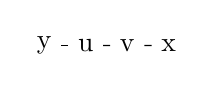
\begin{tikzpicture}
	[style={level distance=1.5em},
	grow=right]
	\node {y}
	child {
		node{u}
		child {
			node{v}
			child {
				node{x}}
		}
	};
	\end{tikzpicture}
	\paragraph{二元函数}
	
	\begin{theorem}
		多元复合函数求\textbf{全导数}
		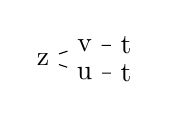
\begin{tikzpicture}
		[style={sibling distance=1em,level distance=1.5em},
		grow=right]
		\node {z}
		child {
			node{u}
			child {
				node{t}
			}
		}
		child {
			node{v}
			child {
				node{t}
			}
		};
		\end{tikzpicture}
		\begin{itemize}
			\item 前提
			\subitem $z=f(u,v)$在$(u_0,v_0)$偏导数连续\quad(z在$(u_0,v_0)$可微分)
			\subitem $u=\varphi(t),v=\psi(t)$在$t_0$偏导数存在
			\item 结果
			\subitem 复合函数$ z=f(\varphi(t),\psi(t)) $在$t_0$可偏导
			\subitem $ \frac{\ud z}{\ud t}=\frac{\partial z}{\partial u}\frac{\ud u}{\ud t}+\frac{\partial z}{\partial v}\frac{\ud v}{\ud t} $
			\item 证明\\
			$
			\begin{array}{rcll}
				\ud z & = & 
				z_u\big|_{\begin{subarray}
					uu = u_0\\
					v = v_0
					\end{subarray}}
					\ud u
					+
				z_v\big|_{\begin{subarray}
					uu = u_0\\
					v = v_0
					\end{subarray}}
					\ud v
					+
					o(\rho)\quad(\rho = \sqrt{(\Delta u)^2+(\Delta v)^2})\\
					
				\lim\limits_{\Delta t \rightarrow 0}\frac{\Delta z}{\Delta t} & = & 
				\lim\limits_{\Delta t \rightarrow 0}
				\frac{\overbrace{z_u\big|_{\begin{subarray}
							uu = u_0\\
							v = v_0
							\end{subarray}}}^{\mbox{与}\Delta u\mbox{无关}}
					\overbrace{\Delta u}^{u=u_0\mbox{附近}}}{\Delta t}
				+
				\lim\limits_{\Delta t \rightarrow 0}
				\frac{z_v\big|_{\begin{subarray}
						uu = u_0\\
						v = v_0
						\end{subarray}}
					\overbrace{\Delta v}^{v=v_0\mbox{附近}}}{\Delta t}
				+
				\lim\limits_{\Delta t \rightarrow 0}
				\frac{o(\rho)}{\underbrace{\rho}_{\rho \rightarrow 0}}\overbrace{\frac{\rho}{\Delta t}}^{\mbox{正负常数}}\\
				
			\end{array}
			$
		\end{itemize}
	\end{theorem}
	\subsection{复合函数的中间变量均为多元函数}
	\begin{theorem}
		多元复合函数求偏导数
		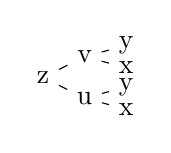
\begin{tikzpicture}
		[level 1/.style={sibling distance=1.5em,level distance=1.5em},
		level 2/.style={sibling distance=0.8em,level distance=1.5em},
		grow=right]
		\node {z}
		child {
			node{u}
			child {
				node{x}
			}
			child {
				node{y}
			}
		}
		child {
			node{v}
			child {
				node{x}
			}
			child {
				node{y}
			}
		};
		\end{tikzpicture}
		\begin{itemize}
			\item 前提
			\subitem $z=f(u,v)$在$(u_0,v_0)$偏导数连续\quad(z在$(u_0,v_0)$可微分)
			\subitem $u=\varphi(x,y),v=\psi(x,y)$在$(x_0,y_0)$偏导数存在
			\item 结果
			\subitem $ \frac{\partial z}{\partial x} = \frac{\partial z}{\partial u}\frac{\partial u}{\partial x}+\frac{\partial z}{\partial v}\frac{\partial v}{\partial x} $
			\subitem $ \frac{\partial z}{\partial y} =
			 \frac{\partial z}{\partial u}\frac{\partial u}{\partial y}+
			 \frac{\partial z}{\partial v}\frac{\partial v}{\partial y} $
		\end{itemize}
	\end{theorem}
	\subsection{复合函数的中间变量有一元函数、多元函数}
	\begin{theorem}
		多元函数求偏导数1
		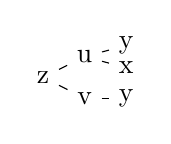
\begin{tikzpicture}
		[level 1/.style={sibling distance=1.5em,level distance=1.5em},
		level 2/.style={sibling distance=0.8em,level distance=1.5em},
		grow=right]
		\node {z}
		child {
			node{v}
			child{
				node{y}
			}
		}
		child {
			node{u}
			child {
				node{x}
			}
			child {
				node{y}
			}
		};
		\end{tikzpicture}
		\begin{itemize}
			\item 前提
			\subitem $u=\varphi(x,y)$在$(x_0,y_0)$偏导数存在$,v=\psi(x)$在$x_0$导数存在
			\subitem $z=f(u,v)$在$(u_0,v_0)$偏导数连续\quad(z在$(u_0,v_0)$可微分)
			\item 结果
			\subitem $\frac{\partial z}{\partial x}=\frac{\partial z}{\partial u}\frac{\partial u}{\partial x}$
			\subitem $\frac{\partial z}{\partial y}=\frac{\partial z}{\partial u}\frac{\partial u}{\partial y}+\frac{\partial z}{\partial v}\frac{\partial v}{\partial y}$
		\end{itemize}
	\end{theorem}

	\begin{theorem}
		多元函数求偏导数2
		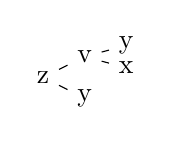
\begin{tikzpicture}
		[level 1/.style={sibling distance=1.5em,level distance=1.5em},
		level 2/.style={sibling distance=0.8em,level distance=1.5em},
		grow=right]
		\node {z}
		child {
			node{y}
		}
		child {
			node{v}
			child {
				node{x}
			}
			child {
				node{y}
			}
		};
		\end{tikzpicture}
		\begin{itemize}
			\item 前提
			\subitem $z=z(x,y)=f(x,v)$
			\item 结果
			\subitem 
			$
			\renewcommand\arraystretch{1.8}
			\begin{array}{ll}
				\frac{\partial z}{\partial x}=
				\frac{\partial f}{\partial v}\frac{\partial v}{\partial x}&f_1'u_x\\
				\frac{\partial z}{\partial y}=
				\frac{\partial f}{\partial u}\frac{\partial u}{\partial y}+
				\frac{\partial f}{\partial y}&f_1'u_y+f_2'\\
			\end{array}
			$
		\end{itemize}
	\end{theorem}
	\subsection{全微分形式不变性}
	中间变量可以写作自变量微分的形式
	\section{隐函数的求导公式}
	\subsection{一个方程的情形}
	\begin{theorem}[隐函数存在定理1]
		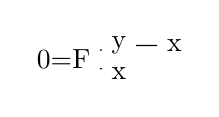
\begin{tikzpicture}
		[style={sibling distance=1em,level distance=2em},
		grow=right]
		\node {0=F}
		child{node{x}}
		child{node{y}child{node{x}}};
		\end{tikzpicture}
		\begin{itemize}
			\item 前提
			\subitem $F(x,y)$在$P(x_0,y_0)$点邻域连续可偏导
			\subitem $F(x_0,y_0)=0$
			\subitem $F_y(x_0,y_0)\neq0$\quad(保号性)
			\item 结果
			\subitem $\exists\mbox{唯一}y=f(x)$偏导连续在$(x,y)$
			\subitem $y_0=f(x_0)$
			\subitem $\frac{\ud y\hla{(\ud f)}}{\ud x}=-\frac{F_x}{F_y}$
			\item \hl{注意此时z不是x的函数}
		\end{itemize}
	\end{theorem}
	\begin{theorem}
		隐函数存在定理2
		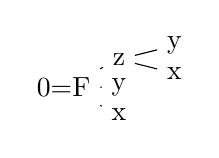
\begin{tikzpicture}
		[style={sibling distance=1em,level distance=2em},
		grow=right]
		\node {0=F}
		child{node{x}}
		child{node{y}}
		child{node{z}
			child{node{x}}
			child{node{y}}
		};
		\end{tikzpicture}
		\begin{itemize}
			\item 前提
			\subitem $F(x,y,z)$在$P(x_0,y_0,z_0)$点邻域连续可偏导
			\subitem $F(x_0,y_0,z_0)=0$
			\subitem $F_y(x_0,y_0,z_0)\neq0$\quad(保号性)
			\item 结果
			\subitem $\exists\mbox{唯一}z=f(x,y)$偏导连续在$(x,y)$
			\subitem $z_0=f(x_0,y_0)$
			\subitem $\frac{\ud z}{\ud x}=-\frac{F_x}{F_z}$
			\subitem $\frac{\ud z}{\ud y}=-\frac{F_y}{F_z}$
		\end{itemize}
	\end{theorem}
	\subsection{方程组的情形}
	\subsubsection{三元方程}
	$\left\{ \begin{array}{l}
	F(x,y,z)=0\\
	\Phi(x,y,z)=0 
	\end{array} \right.$\\
	以x为自由未知量(自变量)\\
	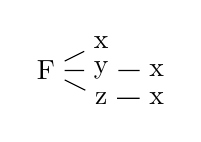
\begin{tikzpicture}
	[style={sibling distance=1em,level distance=2em},
	grow=right]
	\node {F}
	child{node{z}
		child{node{x}}
	}
	child{node{y}
		child{node{x}}
	}
	child{node{x}};
	\end{tikzpicture}
	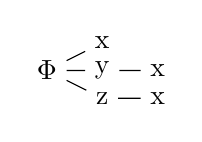
\begin{tikzpicture}
	[style={sibling distance=1em,level distance=2em},
	grow=0]
	\node {$\Phi$}
	child{node{z}
		child{node{x}}
	}
	child{node{y}
		child{node{x}}
	}
	child{node{x}};
	\end{tikzpicture}\\
	同时对两边求x的偏导函数\\
	$
	F_1+F_2y_x+F_3z_x = 0\\
	\Phi_1+\Phi_2y_x+\Phi_3z_x = 0
	$\\
	解方程可求出$z_x,z_y$。
	
		\subsubsection{四元方程}
	$\left\{ \begin{array}{l}
	F(x,y,u,v)=0\\
	\Phi(x,y,u,v)=0 
	\end{array} \right.$\\
	以x,y为自由未知量(自变量)\\
	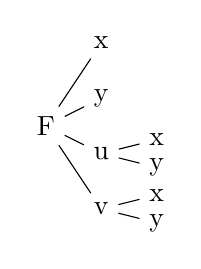
\begin{tikzpicture}
	[level 1/.style={sibling distance=2em,level distance=2em},
	level 2/.style={sibling distance=1em,level distance=2em},
	grow=right]
	\node {F}
	child{node{v}
		child{node{y}}
		child{node{x}}
	}
	child{node{u}
		child{node{y}}
		child{node{x}}
	}
	child{node{y}}
	child{node{x}};
	\end{tikzpicture}
	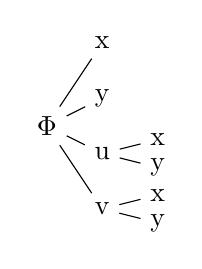
\begin{tikzpicture}
	[level 1/.style={sibling distance=2em,level distance=2em},
	level 2/.style={sibling distance=1em,level distance=2em},
	grow=right]
	\node {$\Phi$}
	child{node{v}
		child{node{y}}
		child{node{x}}
	}
	child{node{u}
		child{node{y}}
		child{node{x}}
	}
	child{node{y}}
	child{node{x}};
	\end{tikzpicture}\\
	同时对两边求x,y的偏导函数\\
	$
	\begin{array}{cc}
	F_1+F_3u_x+F_4v_x = 0& F_2+F_3u_y+F_4v_y = 0 \\ 
	\Phi_1+\Phi_3u_x+\Phi_4v_x = 0 & \Phi_2+\Phi_3u_y+\Phi_4v_y = 0
	\end{array} 
	$\\
	解方程可求出$u_x,u_y,v_x,v_y$。
	\section{多元函数微分学的几何应用}
	\subsection{空间曲线的切线与法平面}
	\subsubsection{预备知识}
	\paragraph{空间曲线的方程}
	\subparagraph{参数式}$\left\{\begin{array}{ll}
	x=\phi(t) &\phi'(t_0)=\lim\limits_{\Delta t \rightarrow 0}\frac{\Delta x(t=t_0\mbox{附近})}{\Delta t}\\ 
	y=\psi(t) \\ 
	z=\omega(t)
	\end{array}\right. $
	\subparagraph{一般式}
	\paragraph{空间直线的方程}
	\subparagraph{点向式(对称式、标准式)}$\frac{x-x_0}{m}=\frac{y-y_0}{n}=\frac{z-z_0}{p}$
	\subparagraph{一般式}	$ \left\{\begin{array}{ll}
	F(x,y,z)=0\quad\mbox{或}\quad A_1x+B_1y+C_1z+D_1=0\\ 
	G(x,y,z)=0\quad\mbox{或}\quad A_2x+B_2y+C_2z+D_2=0
	\end{array} \right. $对应系数不成比例
	\paragraph{空间平面的方程}
	\subparagraph{\hl{点法式}} $A(x-x_0)+B(y-y_0)+C(z-z_0)=0$\quad 法向量$ (A,B,C) $
	\subparagraph{一般式} $Ax+By+Cz+D=0$\quad \hl{法向量$ (A,B,C) $}
	\subparagraph{截距式} $ \frac{x}{a}+\frac{y}{b}+\frac{z}{c}=\hla{1} $\quad 截距$ (a,b,c) $
	\subsubsection{第一种空间曲线(参数式)}
	\subsubsection{切线}
	\paragraph{割线}$MM'$
	\subparagraph{点}$M(x_0,y_0,z_0)$,$M'(x_0+\Delta x,y_0+\Delta y,z_0+\Delta z)$
	\subparagraph{方向向量} $M'-M=(\Delta x,\Delta y,\Delta z)$
	\paragraph{切线}$MM'$
	\subparagraph{点}$M(x_0,y_0,z_0)$,$\lim\limits_{\Delta x \rightarrow 0}M'(x_0+\Delta x,y_0+\Delta y,z_0+\Delta z)$
	\subparagraph{方向向量(切向量)} $\frac{M'-M}{\underbrace{\Delta t}_{\displaystyle\mbox{除以}\Delta t\mbox{对向量无影响}}}=\lim\limits_{\underbrace{\Delta t \rightarrow 0}_{\displaystyle\mbox{就是}\Delta x \rightarrow 0}}
	(\underbrace{\frac{\Delta x}{\Delta t}}_{\displaystyle\phi'(t_0)},\frac{\Delta y}{\Delta t},\frac{\Delta z}{\Delta t})
	\\=\overrightarrow{T}\hla{(\phi'(t_0),\psi'(t_0),\omega'(t_0))}$
	\subparagraph{点向式方程(切线方程)} $\hla{\frac{x-x_0}{\varphi'(t)}=\frac{y-y_0}{\psi'(t_0)}=\frac{z-z_0}{\omega'(t_0)}}$分母可以为0
	\subsubsection{法平面}
	\paragraph{法平面}
	\subparagraph{曲线的切向量,法平面的法向量} $ (\phi'(t_0),\psi'(t_0),\omega'(t_0)) $
	\subparagraph{点} $ M(x_0,y_0,z_0) $
	\subparagraph{点法式方程} $ \phi'(t_0)(x-x_0)+\psi'(t_0)(y-y_0)+\omega'(t_0)(z-z_0)=0 $
	\subsubsection{第二种空间曲线(过渡式)}
	\paragraph{方程}
	$ \left\{\begin{array}{ll}
	[x=x] \\ 
	y=\varphi(x)&\mbox{柱面,母线平行于y轴,准线在XoY平面上} \\ 
	z=\psi(x)&\mbox{柱面,母线平行于z轴,准线在XoZ平面上}
	\end{array} \right. $
	\paragraph{切向量} $\textbf{T}(1,\varphi'(x_0),\psi'(x_0))$
	\paragraph{切线方程} $\hla{\frac{x-x_0}{1}=\frac{y-y_0}{\varphi'(t_0)}=\frac{z-z_0}{\psi'(t_0)}}$
	\subsubsection{第三种空间曲线(一般式)}
	\paragraph{方程}
	$ \left\{\begin{array}{ll}
	[x=x]\\
	F(x,y,z)=0 \\ 
	G(x,y,z)=0 
	\end{array} \right. $
	\paragraph{切向量} $\textbf{T}(1,y'(x_0),z'(x_0))$
	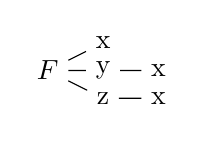
\begin{tikzpicture}
	[style={sibling distance=1em,level distance=2em},
	grow=right]
	\node {$F$}
	child{node{z}
		child{node{x}}
	}
	child{node{y}
		child{node{x}}
	}
	child{node{x}};
	\end{tikzpicture}
	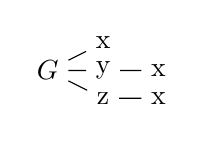
\begin{tikzpicture}
	[style={sibling distance=1em,level distance=2em},
	grow=0]
	\node {$G$}
	child{node{z}
		child{node{x}}
	}
	child{node{y}
		child{node{x}}
	}
	child{node{x}};
	\end{tikzpicture}
	隐函数方程组两边同时对x求导,解方程
	\paragraph{切线方程} $\hla{\frac{x-x_0}{1}=\frac{y-y_0}{y'(x_0)}=\frac{z-z_0}{z'(x_0)}}$
	\subsection{曲面的切平面与法线}
	\subsubsection{预备知识}
	\paragraph{空间曲面的方程}
	\subparagraph{一般方程} $F(x,y,z)=0$
	\paragraph{向量的方向余弦}
	\subparagraph{向量}$ (a_x,a_y,a_z) $
	\subparagraph{方向余弦}$ 
	\cos\alpha = \frac{a_x}{\sqrt{a_x^2+a_y^2+a_z^2}},
	\cos\beta = \frac{a_y}{\sqrt{a_x^2+a_y^2+a_z^2}},
	\cos\gamma = \frac{a_z}{\sqrt{a_x^2+a_y^2+a_z^2}}
	 $
	\paragraph{曲面}
	\subparagraph{一般方程} $F(x,y,z)=0$
	\subsubsection{第一种曲面}
	\paragraph{曲面上的一条曲线}
	\subparagraph{定点} $(x_0,y_0,z_0)$
	\subparagraph{一般方程(任意一条曲线)}$\left\{\begin{array}{l}
	x=x(t) \\ 
	y=y(t) \\ 
	z=z(t)
	\end{array}\right. $
	,$F(x(t),y(t),z(t))\equiv0$
	\subparagraph{方程在定点的全导数} $\begin{array}{l}
	F_1(x_0,y_0,z_0)x'(t_0)+F_2(x_0,y_0,z_0)y'(t_0)+F_3(x_0,y_0,z_0)z'(t_0)=0 \\ 
	(F_1(x_0,y_0,z_0),F_2(x_0,y_0,z_0),F_3(x_0,y_0,z_0))\cdot(x'(t_0),y'(t_0),z'(t_0))=0\\
	\underbrace{(F_1(x_0,y_0,z_0),F_2(x_0,y_0,z_0),F_3(x_0,y_0,z_0))}_{\begin{array}{c}
		\mbox{无论直线方程怎么取} \\ 
		\mbox{它都是一个定值}\\
		\mbox{仅与定点}(x_0,y_0,z_0)\mbox{有关}
		\end{array} }\bot
	\underbrace{(x'(t_0),y'(t_0),z'(t_0))}_{
	\begin{array}{c}
	\mbox{定点切向量} \\ 
	\mbox{是任意曲线的}
	\end{array}
	}
\end{array}$
	\subparagraph{\hl{在定点处的法向量}}$ (F_1(x_0,y_0,z_0),F_2(x_0,y_0,z_0),F_3(x_0,y_0,z_0)) $
	\subparagraph{在定点处的法线方程}$\frac{x-x_0}{F_1(x_0,y_0,z_0)}=\frac{y-y_0}{F_2(x_0,y_0,z_0)}=\frac{z-z_0}{F_3(x_0,y_0,z_0)}$
	\subparagraph{\hl{在定点处的切平面}}$ F_1(x_0,y_0,z_0)(x-x_0)+F_2(x_0,y_0,z_0)(y-y_0)+F_3(x_0,y_0,z_0)(z-z_0)=0 $
	\subsubsection{第二种曲面}
	\paragraph{曲面}
	\subparagraph{特殊方程} $z=f(x,y)$
	\subparagraph{一般方程} $F(x,y,z)=\left\{\begin{array}{c}
	f(x,y)-z \\ 
	\hla{z-f(x,y)}
	\end{array}\right\} =0$
	\subparagraph{\hl{注意}}z对x,y求导等于0,f对x,y求偏导等于偏导
	\paragraph{曲面上的一条曲线}
	\subparagraph{定点} $(x_0,y_0,z_0)$
	\subparagraph{在定点处的法向量}$ (\pm f_1(x_0,y_0),\pm f_2(x_0,y_0),\mp 1) $
	\subparagraph{在定点处的法线方程}$\frac{x-x_0}{\pm f_1(x_0,y_0)}=\frac{y-y_0}{\pm f_2(x_0,y_0)}=\frac{z-z_0}{\mp 1}$
	\subparagraph{在定点处的切平面}$ f_1(x_0,y_0)(x-x_0)+f_2(x_0,y_0)(y-y_0)-1(z-z_0)=0 $
	\subsubsection{切平面的全微分含义}
	\paragraph{切平面方程}$ f_1(x_0,y_0)(x-x_0)+f_2(x_0,y_0)(y-y_0)-\underbrace{1(z-z_0)}_{\displaystyle\Delta z - o(\rho)=\ud z\mbox{的真正含义}}=0 $
	\paragraph{全微分方程}$ f_1(x_0,y_0)\Delta x+f_2(x_0,y_0)\Delta y-\hla{\ud} z=0 $
	\subsubsection{法向量的方向角}
	\paragraph{正常的法向量}$ (\pm f_1(x_0,y_0),\pm f_2(x_0,y_0),\mp 1) $
	\paragraph{向上的法向量}$ (-f_1(x_0,y_0),-f_2(x_0,y_0),1) $
	\paragraph{向上的法向量的方向余弦}$ 
	\cos\alpha = \frac{-f_x}{\sqrt{1+f_x^2+f_y^2}},
	\cos\beta = \frac{-f_y}{\sqrt{1+f_x^2+f_y^2}},
	\cos\gamma = \frac{1}{\sqrt{1+f_x^2+f_y^2}} $
	\section{略}
	\section{多元函数的极值及其求法}
	\subsection{(无条件极值)多元函数的极值及其最大值、最小值}
	\subsubsection{极值}
	\begin{definition}
		二元函数的极大值、极小值
		\begin{itemize}
			\item 前提 $z=f(x,y)$定义域$D$内点$ P_0(x_0,y_0) $
			\item 条件 $ \exists U(P_0)\subset D ,\forall(x,y)\neq(x_0,y_0)$
			\item 结果
			\begin{itemize}
				\item $ f(x,y)>f(x_0,y_0) $\quad 极小值
				\item $ f(x,y)<f(x_0,y_0) $\quad 极大值
			\end{itemize}
		\end{itemize}
	\end{definition}
	\paragraph{驻点与极值}
	\begin{theorem}
		必要条件\hl{(极值具有的性质)}
		\begin{itemize}
			\item 前提
			\begin{itemize}
				\item $ z=f(x,y) $在$ (x_0,y_0) $具有偏导数
				\item $ z=f(x,y) $在$ (x_0,y_0) $具有极值
			\end{itemize}
			\item 结论
			\begin{itemize}
				\item \hl{$ f_x(x_0,y_0)=0 $}
				\item \hl{$ f_y(x_0,y_0)=0 $}
				\item $ (x_0,y_0) $为\hl{驻点}
			\end{itemize}
			\item 推论
			\begin{itemize}
				\item 曲面在$ (x_0,y_0) $的切平面平行于XoY平面
			\end{itemize}
			\item 证明(极大值)\\
			$ 
			\begin{array}{rrr}
			f_x^+(x_0,y_0) & = & \lim\limits_{\Delta x\rightarrow0^+}\frac{f(x_0+\Delta x,y_0)-f(x_0,y_0)\ominus}{\Delta x\oplus} \leqslant 0\\ 
			f_x^-(x_0,y_0) & = & \lim\limits_{\Delta x\rightarrow0^-}\frac{f(x_0+\Delta x,y_0)-f(x_0,y_0)\ominus}{\Delta x\ominus} \geqslant 0\\ 
			f_x(x_0,y_0) & = & \lim\limits_{\Delta x\rightarrow0}\frac{f(x_0+\Delta x,y_0)-f(x_0,y_0)}{\Delta x} = 0\\ 
			\end{array} 
			 $
		\end{itemize}
	\end{theorem}
	\begin{theorem}[充分条件]
		\hl{判断极值的方法}
		\begin{itemize}
			\item 前提
			\begin{itemize}
				\item $ z=f(x,y) $在$ (x_0,y_0) $某邻域连续
				\item $ z=f(x,y) $在$ (x_0,y_0) $两阶偏导函数连续
				\item $ \left\{\begin{array}{c}
				f_x(x_0,y_0)=0 \\ 
				f_y(x_0,y_0)=0
				\end{array}\right\}  \Leftrightarrow(x_0,y_0)$为驻点
				\item $ f_{xx}(x_0,y_0)=A,f_{xy}(x_0,y_0)=B,f_{yy}(x_0,y_0)=C $
			\end{itemize}
			\item 条件
			\begin{enumerate}
				\item $ AC-B^2>0 $
				\item $ AC-B^2<0 $
				\item $ AC-B^2=0 $
			\end{enumerate}
			\item 结论
			\begin{enumerate}
				\item \hl{$ A<0 $为极大值,$ A>0 $为极小值}
				\item 没有极值
				\item 不定
			\end{enumerate}
			\item 证明:不讲
		\end{itemize}
	\end{theorem}
	\paragraph{无偏导点与极值}
	\begin{theorem*}[极值的第二种可能]
		偏导数不存在的点也可能是极值点,比如
		$ z=-\sqrt{x^2+y^2} $
	\end{theorem*}
	\subsubsection{最值(最大值、最小值)}
	\paragraph{存在性}连续函数在闭区域上一定有最大最小值
	\paragraph{可能位置}
	\subparagraph{边界}用边界方程找出y、x的关系,代入原方程,求一元函数最值
	\subparagraph{内部(广义极值点)}
	驻点、偏导数不存在点
	\paragraph{判断方法}
	\begin{enumerate}
		\item 解方程组$ f_{x}(x,y)=0,f_{y}(x,y)=0 $,找无导数点
		\item 对于每一个驻点,求二阶偏导数ABC
		\item 根据$ AC-B^{2} $判断极值情况
	\end{enumerate}
	\subsection{条件极值\quad 拉格朗日乘数法}
	\subsubsection{条件极值}
	\paragraph{代入法}从约束条件中解出z
	对自变量有附加条件的极值
	\subsubsection{拉格朗日乘数法}
	\paragraph{原始条件}
	\subparagraph{目标函数}$ z=f(x,y) $
	\subparagraph{约束条件}$ \varphi(x,y)=\hla{0} $
	\paragraph{推导}
	\[ \begin{array}{rrcl}
	\mbox{假设确定隐函数的显化函数}&y&=&\psi(x)\\
	\mbox{原函数成为x的一元函数}&z&=&f[x,\psi(x)]\\
	\mbox{求全导数}&z_x&=&f_1+f_2\dfrac{\ud \psi}{\ud x}\\
	\mbox{从约束条件求}\dfrac{\ud \psi}{\ud x}&\dfrac{\ud \psi}{\ud x}&=&-\frac{\varphi_{x}}{\varphi_{y}}\\
	\mbox{取得极值时,一元函数(全)导数为0}&0&=&f_1-f_2\frac{\varphi_{x}}{\varphi_{y}}\\
	\mbox{上式变形}&\frac{f_1}{\varphi_x}&=&\frac{f_2}{\varphi_y}\\
	\mbox{设}-\lambda&\frac{f_1}{\varphi_x}&=&\frac{f_2}{\varphi_y}=-\lambda\\
	\mbox{目标条件方程组}&&=&\left\lbrace \begin{array}{l}
	z_x=f_1+\lambda \varphi_x=0\\
	z_y=f_2+\lambda \varphi_y=0\\
	\varphi(x,y)=0
	\end{array}\right. 
	\end{array} \]
	\paragraph{拉格朗日函数}$ L(x,y,\lambda)=f(x,y)+\lambda\varphi(x,y) $
	\subparagraph{拉格朗日乘子}$ \lambda $(可与x,y一起解出,最后不需要)
	\subparagraph{用法}求拉格朗日函数的极值$ \Leftrightarrow $求目标函数(加约束条件)的极值
	\subparagraph{求拉格朗日函数的极值}$ \left\lbrace \begin{array}{rcl}
	F_x&=&f_1+\lambda \varphi_x=0\\
	F_y&=&f_2+\lambda \varphi_y=0\\
	F_\lambda&=&\varphi(x,y)=0
	\end{array}\right.  $
	\subparagraph{消元方法}\hl{移项相除}
	\subparagraph{结果}求出的点是嫌疑点:驻点
	\subparagraph{实际问题}一个驻点就是解
	\subsubsection{拉格朗日乘数法-两个约束条件}
	\paragraph{拉格朗日函数-多约束条件}$ L(x,y,z,\lambda,\mu)=f(x,y,z)+\lambda(x,y,z)+\mu(x,y,z) $
	\chapter{重积分}
	\section{二重积分的概念与性质}
	\subsection{二重积分的概念}
	\paragraph{一重积分}
	$ \lim\limits_{\lambda\rightarrow 0}\sum_{i=1}^{n}
	\underbrace{f(\xi_i)}
	_{\mbox{高}}
	\underbrace{\Delta x}
	_{\mbox{宽}}
	=\int_{a}^{b}f(x)\ud x $
	\subparagraph{注意}不是$ n\rightarrow0 $而是$ \lambda\rightarrow 0 $
	\subparagraph{极限}小区间最大长度
	\subsubsection{曲顶柱体的体积}
	\subsubsection{二重积分}
	$ \lim\limits_{\lambda\rightarrow 0}
	\overbrace{\sum_{i=1}^{n}
		\underbrace{f(\xi_i,\eta_i)}
		_{\mbox{高}}
		\underbrace{\Delta\sigma_i}
		_{\mbox{底面积}}}
	^{\mbox{积分和}}
	=\iint\limits_{D}
	\overbrace{
		\underbrace{f(
			\overbrace{x,y}
			^{\mbox{积分变量}}
			)}
		_{\mbox{被积函数}}
		\ud\sigma}
	^{\mbox{被积表达式}}
	$
	\subparagraph{直径}$\lambda (\Delta {\sigma _k}) = \max \left\{ {\,\left| {\,{P_1}{P_2}\,} \right|\left.  \right|\,{P_1},{P_2} \in \Delta {\sigma _k}} \right\}  $
	\subparagraph{极限}
	$
	\lambda  = \max\limits_{1 \le k \le n} \left\{ {\lambda (\Delta {\sigma _k})} \right\}$
	\subsubsection{平面薄片的质量}
	\subsection{二重积分的性质}
	\begin{property}[线性性质]
	\end{property}
	\begin{property}[区域可加]
		$\iint\limits_{{D_1} \cup {D_2}} {f(x,y)d\sigma } = \iint\limits_{{D_1}} {f(x,y)d\sigma } + \iint\limits_{{D_2}} {f(x,y)d\sigma }.$
	\end{property}
	\begin{property}[求体积]
		$V  = \iint\limits_D {1 \cdot d\sigma  = \iint\limits_D {d\sigma }}.$
	\end{property}
	\begin{property}[不等式性质]
		$f(x,y) \leqslant g(x,y),$\\
		$\iint\limits_D {f(x,y)d\sigma  \leqslant }\iint\limits_D {g(x,y)d\sigma }.$\\
		$\left| {\iint\limits_D {f(x,y)d\sigma }} \right| \leqslant \iint\limits_D {\left| {f(x,y)} \right|d\sigma }.$\quad(上-下$ \leqslant $上+下)
	\end{property}
	\begin{property}[估值不等式]
		设$ M,m $分别是$ \sigma $在闭区域D上的最大值和最小值,$ \sigma $为D的面积,则\\
		\[ m\sigma  \leqslant \iint\limits_D {f(x,y)d\sigma  \leqslant M\sigma } \]
	\end{property}
	\begin{property}[中值定理(要求f连续)]
		$\iint\limits_D {f(x,y)d\sigma } = f(\xi ,\eta ) \cdot \sigma $
	\end{property}
	\subsection{二重积分的计算法}
	\section{三重积分}
	\section{重积分的应用}
	\subsection{曲面的面积}
	$
	\begin{array}{rcll}
		\ud A &=& \dfrac{\ud\sigma}{\cos\gamma}\\
		A &=& \iint\limits_D \dfrac{\ud\sigma}{\cos\gamma}\\
		A &=& \iint\limits_D {\sqrt {1 + f_x^2 + f_y^2} \ud\sigma }
	\end{array}
	$
	\chapter{曲线积分与曲面积分}
	\section{对弧长的曲线积分}
	\subsection{对弧长的曲线积分的概念与性质}
	\subsubsection{概念}
	\paragraph{平面曲线}
	$ \lim\limits_{\lambda\rightarrow 0}
	\overbrace{\sum_{i=1}^{n}
		\underbrace{f(\xi_i,\eta_i)}
		_{\mbox{线密度}}
		\underbrace{\Delta s_i}
		_{\mbox{弧长}}}
	^{\mbox{积分和(式)}}
	=\int_{
		\underbrace{L}
		_{\mbox{积分弧段}}
	}
	\overbrace{
		\underbrace{f(
			\overbrace{x,y}
			^{\mbox{积分变量}}
			)}
		_{\mbox{被积函数}}
		\ud s}
	^{\mbox{被积表达式}}
	$
	\paragraph{空间曲线}
	$ \lim\limits_{\lambda\rightarrow 0}
	\overbrace{\sum_{i=1}^{n}
		\underbrace{f(\xi_i,\eta_i,\zeta_i)}
		_{\mbox{线密度}}
		\underbrace{\Delta s_i}
		_{\mbox{弧长}}}
	^{\mbox{积分和(式)}}
	=\int_{
		\underbrace{\varGamma}
		_{\mbox{积分弧段}}
	}
	\overbrace{
		\underbrace{f(
			\overbrace{x,y,z}
			^{\mbox{积分变量}}
			)}
		_{\mbox{被积函数}}
		\ud s}
	^{\mbox{被积表达式}}
	$
	\subsubsection{性质}
	\begin{property}[线性性质]
	\end{property}
	\begin{property}[不等式性质]
	\end{property}
	\begin{property}[积分区域的可加性]
	\end{property}
	\begin{property}[定义域]
		定义域是L上的一切点
	\end{property}
	\begin{property}[求弧长]
		被积函数恒等于1
	\end{property}
	\subsection{对弧长的曲线积分的计算法}
	\begin{theorem}[第一类曲线积分的计算]
		计算
		\begin{itemize}
			\item 前提\quad$ \beta\geqslant\alpha $
			\item 结果\quad$ \int_L {f(x,y) \ud s}  = \int_\alpha ^\beta  f[\phi (t),\psi (t)]
				\underbrace{\sqrt {{{\phi '}^2}(t) + {{\psi '}^2}(t)}  \ud t}
			_{\mbox{弧微分}}
			$
		\end{itemize}
	\end{theorem}
	\section{对坐标的曲线积分}
	\subsection{对坐标的曲线积分的概念与性质}
	\subsubsection{概念}
	\begin{definition}定义
		\begin{itemize}
			\item 前提
			\begin{itemize}
				\item L为\hl{有向}光滑曲线弧
				\item L上定义了向量函数$ \overrightarrow{F}=(P(x,y),Q(x,y))  $
			\end{itemize}
		\item 结果
		\begin{itemize}
			\item $ \lim\limits_{\lambda\rightarrow0}\sum_{k=1}^{n}[\overrightarrow{F}(\xi _k,\eta _k) \cdot \overrightarrow{{M_{k - 1}}{M_k}}] $
			\item $ \lim\limits_{\lambda\rightarrow0}\sum_{k=1}^{n}[P({\xi _k},{\eta _k})\Delta {\kern 1pt} {x_k} + Q({\xi _k},{\eta _k})\Delta {\kern 1pt} {y_k}] $
			\item $\int_L {P(x,y){\kern 1pt} d{\kern 1pt} x + Q(x,y)\ud y} $
		\end{itemize}
		\end{itemize}
	\end{definition}
	\subsubsection{性质}
	\begin{property}[线性性质]
	\end{property}
	\begin{property}[区间可加性]
	\end{property}
	\begin{property}[反向弧]
	\end{property}
	\begin{property}[特例]
		定积分
	\end{property}
	\subsection{对坐标的曲线积分的计算法}
	\begin{theorem}计算法
		\begin{itemize}
			\item 前提
			\begin{itemize}
				\item L的参数方程$ \left\lbrace \begin{array}{l}
				x=\varphi(t)\\
				y=\psi(t)
				\end{array}\right.t\in(\alpha\rightarrow\beta)  $
			\end{itemize}
			\item 结果$  =\int_\alpha ^\beta \left\{ P[\varphi (t),\psi (t)] \varphi '(t) + Q\,[\varphi (t),\psi (t)]\psi '(t)    \right\}\ud t$
		\end{itemize}
	\end{theorem}
	\subsection{两类曲线积分之间的联系}
	$\int_L {Pdx + Qdy = } \int_L {(P\cos \alpha  + Q\cos \beta )ds} $\\
	$ \cos\alpha,\cos\beta $的符号包含了第一类的方向(切向量的方向)\\
	$ \ud s = \dfrac{\ud x}{\cos\alpha} $
	\section{格林公式及其应用}
	
	\subsection{格林公式}
	\subsubsection{与一元函数莱布尼茨的联系}
	\subsubsection{单连通区域和复连通区域}
	\paragraph{单连通区域}没有洞
	\paragraph{复连通区域}有洞
	\subsubsection{平面区域的边界的正向}
	人沿曲边走,区域在左手
	\subsubsection{格林公式}
	\begin{theorem}[格林公式]
		格林公式
		\begin{itemize}
			\item 前提
			\begin{itemize}
				\item 闭区域D,分段光滑曲线L
				\item 函数P,Q一阶偏导连续
			\end{itemize}
			\item 结果
			\begin{itemize}
				\item $\iint\limits_D {(\frac{{\partial Q}}{{\partial x}} - \frac{{\partial P}}{{\partial y}})dxdy} = \oint_L {Pdx + Qdy} $\hl{正向}
				\item $\iint\limits_D {\left| {\begin{array}{*{20}{c}}
						{\frac{\partial }{{\partial x}}}&{\frac{\partial }{{\partial y}}} \\ 
						P&Q 
						\end{array}} \right|}dxdy = \oint_L {Pdx + Qdy} $
			\end{itemize}
			\item 证明
			\begin{enumerate}
				\item $
				\iint_{D}
				\left(\frac{\partial Q}{\partial x} - \frac{\partial P}{\partial y}\right)\ud x \ud y  
				=\oint_{L}	P \ud x + Q \ud y
				$
				\item 
				把P看成0函数\\
				$
				\iint_{D}
				\left(\frac{\partial Q}{\partial x}\right)\ud x \ud y 
				=\oint_{L}	Q \ud y
				$
				\item 
				抽象函数写不出原函数\\
				先对X积分后对Y积分\\
				$
				\iint_{D}
				\left(\frac{\partial Q}{\partial x} \ud x \right)\ud y 
				=\oint_{L}	Q \ud y
				$
				\item 
				二重积分化为一重积分\\
				$
				\int_{c}^{d}\ud y
				\int_{\varphi_{1}(y)}^{\varphi_{2}(y)}\frac{\partial Q}{\partial x} \ud x
				=\oint_{L}	Q \ud y
				$
				\item 
				展开$\ud x$\\
				$
				\int_{c}^{d}Q\left(\varphi_{2}(y),y\right)\ud y - \int_{c}^{d}Q\left(\varphi_{1}(y),y\right)\ud y
				=\oint_{L}	Q \ud y
				$
				\item 
				定积分化为曲线积分\\
				$
				\int_{\arc{CBE}}Q\left(x,y\right) \ud y - \int_{\arc{CAE}}Q\left(x,y\right) \ud y
				=\oint_{L}	Q \ud y
				$
				\item 
				翻转CAE\\
				$
				\int_{\arc{CBE}}Q\left(x,y\right) \ud y + \int_{\arc{EAC}}Q\left(x,y\right) \ud y
				=\oint_{L}	Q \ud y
				$
				\item 
				曲线积分合并\\
				$
				\oint_{L}Q\left(x,y\right) \ud y 
				=\oint_{L}	Q \ud y
				$
			\end{enumerate}
		\end{itemize}
	\end{theorem}
	\subsubsection{格林公式的简单应用}
	\paragraph{求面积}$A = \frac{1}{2}\oint_L {xdy - ydx} $
	\paragraph{求面积}$A = \frac{1}{2}\oint_L {-ydx + xdy} $
	\paragraph{求面积}$A = \oint_L {xdy} $
	\paragraph{求面积}$A = \oint_L {- ydx} $
	\subsection{平面上曲线积分与路径无关的条件}
	\begin{theorem}[充要条件]路径无关
		\begin{itemize}
			\item 前提
			\begin{itemize}
				\item 一阶偏导连续
				\item 单连通域
			\end{itemize}
			\item 结果\quad 路径无关$\Leftrightarrow$$\frac{{\partial P}}{{\partial y}} = \frac{{\partial Q}}{{\partial x}}$
			\item 证明\quad 老师没讲
		\end{itemize}
	\end{theorem}
\begin{enumerate}
	\item 表示 \\$
	\oint_{L}P\ud x + Q \ud y
	=
	\int_{(x_{0},y_{0})}^{(x,y)}P\ud x + Q \ud y
	=
	u(x,y)
	$\\
	$
	\ud u = P\ud x + Q \ud y
	$
	
\end{enumerate}
	\subsection{二元函数的全微分求积} 
%	~{}\\
	\begin{theorem}[充要条件]
		全微分
		\begin{itemize}
			\item 前提
			\item 结果\quad $\frac{{\partial P}}{{\partial y}} = \frac{{\partial Q}}{{\partial x}}\Leftrightarrow\ud u(x,y)=u_x + u_y=P(x,y)\ud x + Q(x,y) \ud y$
			\item 证明\\
			已知 $
			u(x,y)
			=
			\int_{(x_{0},y_{0})}^{(x,y)}P(x,y)\ud x + Q(x,y) \ud y
			$
			\\
			证明
			$
			\ud u(x,y)
			=
			\frac{\partial u(x,y)}{\partial x} + \frac{\partial u(x,y)}{\partial y}
			=
			P(x,y)\ud x + Q(x,y) \ud y
			$\\
			只证
			$
			\frac{\partial u(x,y)}{\partial x}
			=
			P(x,y)\ud x
			$
			\begin{enumerate}
				
				\item 
				$
				P(x,y) =
				\lim\limits_{\Delta x \rightarrow 0}\frac{u(x+\Delta x,y)-u(x,y)}{\Delta x}
				$
				\item 使用已知公式 $
				u(x,y)
				=
				\int_{(x_{0},y_{0})}^{(x,y)}P(x,y)\ud x + Q(x,y) \ud y
				$\\
				$
				P(x,y) =
				\lim\limits_{\Delta x \rightarrow 0}\frac{
					\int_{\hlc{(x_{0},y_{0})}}^{(x+\Delta x,y)}P(x,y)\ud x+ Q(x,y)\ud y
					-
					\int_{\hlc{(x_{0},y_{0})}}^{(x,y)}P(x,y)\ud x+ Q(x,y)\ud y
				}
				{\Delta x}
				$
				\item 合并曲线积分\\
				$
				P(x,y) =
				\lim\limits_{\Delta x \rightarrow 0}\frac{
					\int_{(x,\hlc{y})}^{(x+\Delta x,\hlc{y})}P(x,y)\ud x+ Q(x,y)\ud y
				}\displaystyle
				{\Delta x}
				$
				\item 积分上下限的y没变, $Q(x,y)\ud y$为0\\
				$
				P(x,y) =
				\lim\limits_{\Delta x \rightarrow 0}\frac{
					\int_{\hlc{x}}^{\hlc{x+\Delta x}}P(x,y)\ud x
				}
				{\Delta x}
				$
				\item \hl{定积分中值定理}\\
				$
				P(x,y) =
				\lim\limits_{\Delta x \rightarrow 0}\frac{
					P(
					\hlb{x+\theta \Delta x}
					,y) \Delta x
				}
				{\Delta x}
				$
				$(x<x+\theta \Delta x<x+ \Delta x)$
				\item 消去$\Delta x$\\
				$
				P(x,y) =
				\lim\limits_{\Delta x \rightarrow 0}
				P(x+\theta \Delta x,y)
				$
				\item 取极限
				$
				P(x,y) =
				P(x,y)
				$
			\end{enumerate}
		\end{itemize}
	\end{theorem}
	\section{对面积的曲面积分}
	\subsection{对面积的曲面积分的概念与性质}
	\subsubsection{概念}
	\begin{definition}
		第一类曲面积分
		\begin{itemize}
			\item 前提
%			\item 结果\quad $\mathop {\lim }\limits_{\lambda  \to 0} \sum\limits_{i = 1}^n {f({\xi _i}} ,{\eta _i},{\zeta _i})\Delta {S_i} = \iint\limits_\Sigma  {f(x,y,z)dS}$
			\item 结果\quad
			$ \lim\limits_{\lambda\rightarrow 0}
			\overbrace{\sum_{i=1}^{n}
				\underbrace{f(\xi_i,\eta_i,\zeta _i)}
				_{\mbox{面密度}}
				\underbrace{\Delta S_i}
				_{\mbox{面积元素}}}
			^{\mbox{积分和}}
			=\iint\limits_{
				\underbrace{\scriptstyle\sum}
				_{\mbox{积分曲面}}
			}
			\overbrace{
				\underbrace{f(
					\overbrace{x,y,z(x,y)}
					^{\mbox{积分变量}}
					)}
				_{\mbox{被积函数}}
				\ud S}
			^{\mbox{被积表达式}}
			$
			\item 二重积分\quad
			$ \lim\limits_{\lambda\rightarrow 0}
			\overbrace{\sum_{i=1}^{n}
				\underbrace{f(\xi_i,\eta_i)}
				_{\mbox{高}}
				\underbrace{\Delta\sigma_i}
				_{\mbox{底面积}}}
			^{\mbox{积分和}}
			=\iint\limits_{D}
			\overbrace{
				\underbrace{f(
					\overbrace{x,y}
					^{\mbox{积分变量}}
					)}
				_{\mbox{被积函数}}
				\ud\sigma}
			^{\mbox{被积表达式}}
			$
		\end{itemize}
	\end{definition}
	\subsubsection{性质}
	\begin{property}[线性性质]
	\end{property}
	\begin{property}[积分区域可加性]
	\end{property}
	\begin{property}[存在性]
		$ f(x,y,z) $连续
	\end{property}
	\begin{property}[算表面积]
		$\iint\limits_{\sum } 1\ud S =S$
	\end{property}
	\subsection{对面积的曲面积分的计算法}
	\paragraph{口诀}一代二换三投影
	\paragraph{公式}
	$\iint\limits_{\sum } f(x,y,z)\ud S = \iint\limits_{{D_{xy}}} {f[x,y,z(x,y)]\sqrt {1 + {{z'}_x}^2 + {{z'}_y}^2} }\ud x \ud y$
	\section{对坐标的曲面积分}
	\subsection{对面积的曲面积分的概念与性质}
	\subsubsection{曲面分类}
	\paragraph{双侧曲面}是有向曲面
	\paragraph{单侧曲面}
	\subsubsection{侧的规定}
	\paragraph{前后侧}$ \cos\alpha\quad\ud y\ud z$
	\paragraph{右左侧}$ \cos\beta\quad\ud x\ud z$
	\paragraph{上下侧}$ \cos\gamma\quad\mbox{OZ正向}\quad\ud x\ud y$
	\paragraph{内外侧}封闭曲面
	\subsubsection{有向曲面的投影}
	\paragraph{正常}$ \cos>0 $
	\paragraph{负号}$ \cos<0 $
	\paragraph{零}$ \cos=0 $
	\begin{definition}
		定义\begin{itemize}
			\item 前提
			\item 结果
			\begin{itemize}
				\item 第一类\quad
				$ \lim\limits_{\lambda\rightarrow 0}
				\overbrace{\sum_{i=1}^{n}
					\underbrace{f(\xi_i,\eta_i,\zeta _i)}
					_{\mbox{面密度}}
					\underbrace{\Delta S_i}
					_{\mbox{面积元素}}}
				^{\mbox{积分和}}
				=\iint\limits_{
					\underbrace{\scriptstyle\sum}
					_{\mbox{积分曲面}}
				}
				\overbrace{
					\underbrace{f(
						\overbrace{x,y,z(x,y)}
						^{\mbox{积分变量}}
						)}
					_{\mbox{被积函数}}
					\ud S}
				^{\mbox{被积表达式}}
				$
				\item 第二类\quad
				$ \lim\limits_{\lambda\rightarrow 0}
				\overbrace{\sum_{i=1}^{n}
					\underbrace{R(\xi_i,\eta_i,\zeta _i)}
					_{\mbox{}}
					\underbrace{(\Delta S_i)_{xy}}
					_{\mbox{}}}
				^{\mbox{积分和}}
				=\iint\limits_{
					\underbrace{\scriptstyle\sum}
					_{\mbox{积分曲面}}
				}
				\overbrace{
					\underbrace{R(
						\overbrace{x,y,z(x,y)}
						^{\mbox{积分变量}}
						)}
					_{\mbox{被积函数}}
					\underbrace{\ud S}
					_{\mbox{有向面积元}}
				}
				^{\mbox{被积表达式}}
				$
				\item $\lim\limits_{\lambda  \to 0} \sum\limits_{i = 1}^n {P(\xi_i,\eta_i,\zeta_i){{(\Delta S_i)}_{yz}}}
				=
				\iint\limits_\Sigma  {P(x(y,z),y,z)\ud y\ud z} $
				\item $\lim\limits_{\lambda  \to 0} \sum\limits_{i = 1}^n {P(\xi_i,\eta_i,\zeta_i){{(\Delta S_i)}_{xz}}}
				=
				\iint\limits_\Sigma  {P(x,y(x,z),z)\ud x\ud z} $
			\end{itemize}
		\end{itemize}
	\end{definition}
	\subsubsection{性质}
	\begin{property}[线性性质]
	\end{property}
	\begin{property}[区域可加性]
	\end{property}
	\begin{property}[反向性]
	\end{property}	
	\subsection{对面积的曲面积分的计算法}
	\paragraph{口诀}一代二投三定号
	\subsection{两类曲面积分之间的联系}
	\paragraph{法向量的方向}法向量的方向对应面的方向
	\paragraph{\hl{公式}}$\iint\limits_\Sigma  {Pdydz + Qdzdx + R}dxdy = \iint\limits_\Sigma  {(P\cos \alpha  + Q\cos \beta  + R}\cos \gamma )dS$
	\chapter{无穷级数}
	\section{常数项级数的概念和性质}
	\section{常数项级数的审敛法}
	\section{幂级数}
	\section{函数展开成幂级数}
	\subsection{泰勒级数}
	\subsection{函数展开成幂级数}
	\subsubsection{常用函数的泰勒级数}
	\begin{enumerate}
		\item $\displaystyle
		e^x=\sum_{n=0}^{\infty}\frac{x^n}{n!}$
		\item $\displaystyle
		\sin x = \sum_{n=0}^{\infty}\frac{(-1)^n}{(2n+1)!}x^{2n+1}$
		\item $\displaystyle
		\cos x = \sum_{n=0}^{\infty}\frac{(-1)^n}{(2n)!}x^{2n}$
		\item $\displaystyle
		\frac{1}{1+x} = \sum_{n=0}^{\infty}(-1)^nx^n$
		\item $\displaystyle
		\ln(1+x) = \sum_{n=1}^{\infty}\frac{(-1)^{n-1}}{n}x^n$
		\item $(1+x)^m$
		\subitem $\displaystyle\sqrt{1+x} = 1 + \frac{1}{2}x + \sum_{n=2}^{\infty}(-1)^{n-1}\frac{(2n-3)!!}{(2n)!!}x^n$
		\subitem $\displaystyle
		\frac{1}{\sqrt{1+x}} = 1 + \sum_{n=1}^{\infty}(-1)^{n}\frac{(2n-1)!!}{(2n)!!}x^n$
	\end{enumerate}
	\section{略}
	\section{略}
	\section{傅里叶级数}
	\subsection{三角级数、三角级数系的正交性}
	\subsection{函数展开成傅里叶级数}
	\subsubsection{周期为$2\pi$的函数}
	\subsubsection{收敛定理,狄利克雷充分条件}
	\subsubsection{定义在$[-\pi,\pi]$上的函数}
	\subsubsection{特殊级数的和}
	\subsection{正弦级数和余弦级数}
	\subsubsection{周期为$2\pi$的函数}
	\paragraph{预备知识}
	\subparagraph{奇函数、偶函数}奇$\times$奇=偶,奇$\times$偶=奇,偶$\times$偶=偶
	\subsubsection{定义在$[0,\pi]$上的函数}

\end{document}
